\documentclass[a4paper, 11pt]{article}
\usepackage[utf8]{inputenc}
\usepackage[french]{babel}
\usepackage{amssymb}
\usepackage{amsmath}
\usepackage{graphicx} %pour les images
\usepackage{hyperref} %pour les liens
%\renewcommand*{\familydefault}{\sfdefault} %sans serif
\hypersetup{
    hidelinks=true,
    linktoc=all
}

\title{Travail 1: Système de gestion des employés d’une entreprise}
\author{Julien Stilmant\\\texttt{14054} \and Thierry Frycia\\\texttt{14212}}
\date{\today}

\usepackage{graphicx}
\begin{document}

\maketitle

\section{Structure}
\subsection{Diagramme}
\begin{figure}[htp]
\centering
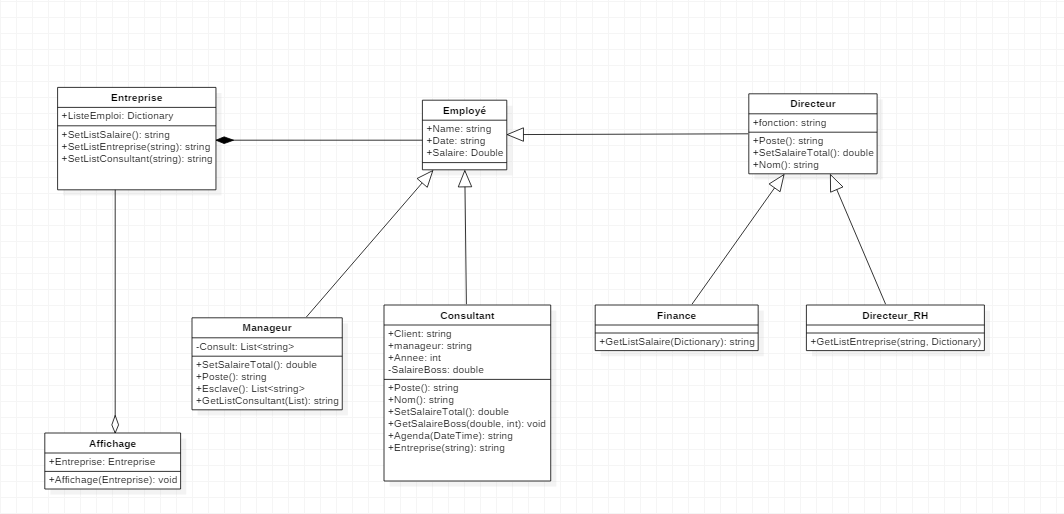
\includegraphics[width=\textwidth]{uml.png}
\end{figure}

\subsection{Fonctionnement du code}
\subsubsection{Structure générale}
La fonction \texttt{Main()} qui se trouve dans la classe \texttt{MainClass} dans le fichier \texttt{Execution.cs} appelle la fonciton \texttt{Emploi()} qui est définie juste en dessous. Cette fonction va lire le contenu des fichiers json, l'interprète et mémorise les données dans les objets du type aproprié. 

Après ça, la fonction \texttt{Affichage()} est appellée avec en paramètre le dictionnaire qui contient tous les objets déserialisés auparavant. C'est cette fonction qui fait l'interface avec l'utilisateur et qui va par après appeler les méthodes appropriés sur les objets pour obtenir leurs attributs.

\subsubsection{Classes principales}
\paragraph{Consultant}
La classe \texttt{Consultant} est une sous-classe de \texttt{Employé}. Elle hérite donc simplement des attributs \texttt{Name}, \texttt{Date} et \texttt{Salaire}. En plus de ça, elle génère des attributs personnels \texttt{Client} et \texttt{manageur}.

Le calcul du salaire se fait dans la méthode \texttt{SetSalaireTotal}, qui vérifie si les missions ont été faites dans une boîte externe ou non et prends en compte le salaire du manager.

\paragraph{Directeurs}
\verb|Directeur_RH| et \texttt{Finance} héritent tous les deux de la classe \texttt{Directeur} qui définit les attributs pour la fonction et le salaire de la personne.

La classe \verb|Directeur_RH| contient une méthode \texttt{GetListEntreprise()} qui renvoie les noms et les dates des consultants qui ont travaillé dans une certaine entreprise. Cette méthode sera appelé par la méthode \texttt{ListConsultants()} dans la classe \texttt{Entreprise}.

Le même principe est utilisé pour la méthode \texttt{GetListSalaire()} du directeur des finances.

\paragraph{Manageur}
Les deux méthodes principales de cette classe sont \texttt{SetSalaireTotal()} et \texttt{GetListConsultant()}.

La première calcule le salaire en fonction du nombre de consultants sous sa responsabilité.

La deuxième est utilisée par la méthode \texttt{SetListConsultants()} dans la classe \texttt{Entreprise} pour générer le rapport du manageur de la même façon que pour les directeurs.

\paragraph{Entreprise}
\texttt{SetSalaire()} envoie le salaire des manageurs à leurs consultants pour que ceux-ci puissent calculer leur salaire.

\texttt{DirecteurFinance()}, \texttt{DirecteurRH()} et \texttt{NomManageur()} renvoient le nom de la personne pour pouvoir l'afficher au final.

\texttt{SelListSalaire()} SelListSalaire envoie à la classe \texttt{Finance} un dictionnaire des noms et des salaires pour que l'intance de cette classe puisse renvoier la liste des salaires.

\texttt{SelListEntreprise} envoie à la classe \verb|Directeur_RH| un dictionnaire des noms et des dates pour que l'intance de cette classe puisse renvoier la liste des consultants travaillant dans une entreprise donnée.

\texttt{SelListConsultant} envoie à la classe \texttt{Manageur} une liste des noms des consultants et de lentreprise où ils travaillent pour que l'intance de cette classe puisse renvoyer cette liste.

\section{Fichiers}
Toutes les données sont stockées dans des fichiers texte au format \texttt{json} séparés selon le poste ou la fonction.

\begin{description}
  \item[Dataadress.json] Contient la liste des emplacements des fichiers \texttt{json} correspondant aux employés.
  \item[Dataemployé.json] Contient une liste de dictionnaires chacun reprenant le nom, le poste, la date de naissance, le salaire et une liste des personnes associés.
  \item[Data(nom).json] Chaque fichier représente un consultant et contient la liste de ses missions avec leur date de début et de fin.
\end{description}



\end{document}